\documentclass[10pt,a4paper]{article}
\usepackage[margin=2.1cm]{geometry}
\usepackage{fontspec}
\usepackage{float}
\usepackage{graphicx,booktabs,array,xcolor,enumitem,titlesec,caption,tabularx,microtype}
\usepackage[colorlinks=true,urlcolor=blue!55!black,linkcolor=black]{hyperref}
\setlength{\parindent}{0pt}\setlength{\parskip}{5pt}
\titleformat{\section}{\large\bfseries}{\thesection}{0.6em}{}
\titleformat{\subsection}{\normalsize\bfseries}{\thesubsection}{0.6em}{}
\titlespacing*{\section}{0pt}{10pt}{3pt}\titlespacing*{\subsection}{0pt}{7pt}{2pt}
\captionsetup{font=small,labelfont=bf}
\setlist{itemsep=1pt,topsep=2pt,leftmargin=1.4em}
\newcommand{\code}[1]{{\small\texttt{#1}}}
\newcommand{\up}{$\rightarrow$}
% Values filled in from the results files.
\newcommand{\NullMin}{11\%}
\newcommand{\NullMinB}{22\%}
\newcommand{\QwenThreeDel}{2}
\newcommand{\PrefixLastRow}{Danish & after a Swedish prefix & $-3.8$ & $+28.0$ & $+3.76$ [$+2.00$, $+5.71$] & $-0.50$ [$-1.48$, $+0.34$] & $-0.09$\\}
\newcommand{\STwoRow}{}
\newcommand{\STwoText}{Pending.}
\newcommand{\ReproText}{Pending.}
\newcommand{\CSixOutcome}{Pending}

\begin{document}

{\LARGE\bfseries\raggedright Weight-only screening finds neurons that control Danish output. Deleting them does not make a model answer in Swedish.\par}
\vspace{4pt}
{\large A two-round, pre-registered test of weight-space programming for Swedish language models\par}
\vspace{4pt}
Jafar Banar \quad$\cdot$\quad 19 November 2026 \quad$\cdot$\quad Report for SE.LLMA

\vspace{4pt}\hrule\vspace{6pt}

\textbf{Summary.}
I tested whether reading a model's weights, without running it, can find and remove the cause of a Swedish-language failure.
On \code{Qwen2.5-1.5B-Instruct} the screen nominated two neurons, and deleting either changes the language of the answers, in opposite directions.
The pre-registered edit (delete both) missed its criteria. A one-neuron edit found afterwards looked strong, but in a second pre-registered round on fresh data
it barely changed how often the model answers in Swedish, and it damaged Danish output in every model tested.
The failure it targets depends on the prompts: on human-translated questions the model answers in English, not Danish, about half the time, and a one-line prompt fixes most of that.
I recommend that SE.LLMA not use weight edits to improve Swedish, and that it measure correct answers in the requested language on its own checkpoints.

\begin{table}[H]\small\centering
\begin{tabularx}{\textwidth}{@{}>{\raggedright\arraybackslash}p{3.1cm}X@{}}
\toprule
Stage & What the result establishes\\
\midrule
\textbf{Round 1, pre-registered} & The two-neuron edit missed its criteria: Swedish answers 85.0\%\up91.2\%, $+6.2$ points, 95\% interval $[-4.7,+18.8]$; Swedish perplexity $+8\%$.\\
\textbf{Round 1, exploratory} & The two single-neuron deletions had large, opposite effects (96.9\% and 20.0\% Swedish answers). These are discovery estimates from data already inspected; their intervals do not account for the selection.\\
\textbf{Round 2, pre-registered} & On new templates the unedited model was below the pre-set 5\% failure gate (3.4\%), so repair could not be tested there. On human-translated questions the one-neuron edit changed Swedish answers 50.0\%\up51.0\%. The Danish-output regression recurred (47.3\%\up16.0\%), and recurred in three further models.\\
\bottomrule
\end{tabularx}
\caption{Chronology. Rounds are separated because the evidence they give is of different kinds.}\label{tab:chrono}
\end{table}

\section{What the article shows, and what it does not}

\emph{Sparks of Weight-Space Programming} (Takehi, Teoh, Zhang and Khattab, November 2026) reports eight experiments in which a frontier LLM (``Astra'') reads or writes
neural-network weights. Table~\ref{tab:critique} sorts them by how much model feedback the LLM had, which is the distinction the assignment asks about.

\begin{table}[H]\small\centering
\begin{tabularx}{\textwidth}{@{}l>{\raggedright\arraybackslash}p{3.3cm}>{\raggedright\arraybackslash}p{3.6cm}>{\raggedright\arraybackslash}X@{}}
\toprule
Exp. & Result & Model feedback available & How strong is the evidence?\\
\midrule
1, 2 & Names the game / shape a small MLP was trained on & None. Weights as text & Weak. 3--4 networks, few-way choice, and first and last layers that are spatial maps.\\
3 & Finds the copying heads in three 7M-parameter transformers & None. Python on weights only & \textbf{Strong for reading.} 24 heads per model against a ground truth the LLM never saw. It applies a published method, on small character-level models, with labels from one probe.\\
4, 5 & One-shot fix of a control policy; MinAtar policies from scratch & None. No tools & \textbf{Strong for writing small programs.} 0\%\up100\% over 1,024 episodes cannot be noise. The tasks have short known algorithms.\\
6 & Go network, 1.5M weights & 0 to 50 batches of 128 games, ``keeps a change only if it wins more'' & Mixed. With feedback this is hill-climbing with an LLM proposing the moves.\\
7 & Which fine-tune is sycophantic? & Weights only: \textbf{fails}. With attention patterns: succeeds & An honest negative for auditing from weights alone.\\
8 & Qwen3.5-0.8B MATH-500 7.9\%\up48.1\% by editing 0.016\% of weights & 50 forward-pass batches incl.\ activations; 158 turns, 80 Python runs, 20 hours & A feedback-informed repair. The design cannot say how much weight reasoning contributed.\\
\bottomrule
\end{tabularx}
\caption{The article's experiments by available feedback. Run details for Experiment 8 are from the authors' released logs.}\label{tab:critique}
\end{table}

\textbf{The headline result removes an obstacle.} 93\% of baseline answers ran into the 32,768-token limit, so the base score measures looping. The authors say so, and their follow-up on Gemma, which rarely loops, found no gain.
Three points limit what it shows about \emph{reasoning about weights}:
\begin{itemize}
\item \textbf{Weight analysis and feedback are confounded.} The 10-, 25- and 50-pass runs each produced a different edit, with one run per budget, so there is no dose--response for one method and no variance estimate.
\item \textbf{The missing comparison is budget-matched.} The unedited model under the same sampling is a control. What is absent is a random edit, and a search or editing baseline (steering, fine-tuning, an inference setting) given the same 50 batches.
\item \textbf{A small edit is not a safe edit.} The article argues that touching 0.016\% of weights can leave the rest of the model intact. Below, an edit to 0.0001\% of the weights flips two thirds of a model's Swedish answers into Danish or Norwegian.
\end{itemize}
\textbf{Justified:} a frontier LLM can compile known algorithms into small networks, execute interpretability recipes on weights, and with feedback remove an obstacle that hides an existing ability.
\textbf{Not justified:} that such edits add capabilities, that models can be audited without evaluation (Experiment 7 failed at this), or that the language-model result came from reading weights.

\section{Question and hypothesis}

\textbf{Finding a failure first.} On development prompts \code{Qwen2.5-1.5B-Instruct} answered 14--19\% of plain Swedish prompts in Danish or Norwegian, for example
``Yttrandefrihet er en vigtig rettighed i mange lande''. Adding ``Svara alltid på svenska.'' removed this on 48 of 48 prompts, so the model can answer in Swedish.

\textbf{Question.} Can a tiny weight edit, found by reading the weights alone, remove this wrong-language behaviour without other damage?

\textbf{Why it matters.} For SE.LLMA this is a direct failure of linguistic precision that perplexity and grammar benchmarks do not see. For the article it is the best case: an existing ability, a narrow failure, a small open model.

\textbf{Round-1 predictions} (\code{PREREGISTRATION.md}, committed before any edit was run). H1: some edit in the family at least halves held-out wrong-language answers, beats random edits, raises Swedish and English perplexity by at most 5\%, and loses at most 2.5 points of English answers.
H2: the edit built with zero forward passes already does so (my prior: 30\%). H3: no edit improves Swedish grammar-pair accuracy by more than 3 points or perplexity by more than 2\%. H4 (diagnostic): if Danish prompts stop getting Danish answers, the edit suppressed a language and did not fix a choice.

\section{Method}

\textbf{Model.} \code{Qwen/Qwen2.5-1.5B-Instruct}, revision \code{989aa798}, Apache-2.0, 28 layers, 8,960 MLP neurons per layer. Half precision on an Apple M3 Pro laptop. Greedy decoding, 48 new tokens, default system prompt, seed 0.

\textbf{Screen with zero forward passes.} The model ties its input and output embeddings. I averaged the embedding differences of 17 Swedish / Danish-Norwegian function-word pairs
(\emph{och/og}, \emph{inte/ikke}, \emph{jag/jeg}, \dots), passed the result through the final normalisation gain, and scored each of the 250,880 MLP neurons by how strongly its output weights point along that direction (a z-score within its layer).
Two neurons scored lowest (Figure~\ref{fig:read}): layer 23 neuron 981 ($z=-9.2$), whose weights promote `` kvinder'', `` søger'', `` danmark'' and suppress ``Ö'', ``ä''; and layer 22 neuron 1821 ($z=-7.9$), which promotes ``ø'', `` Danish'', ``.dk'' and suppresses `` och'', `` ett''.

\begin{figure}[H]\centering
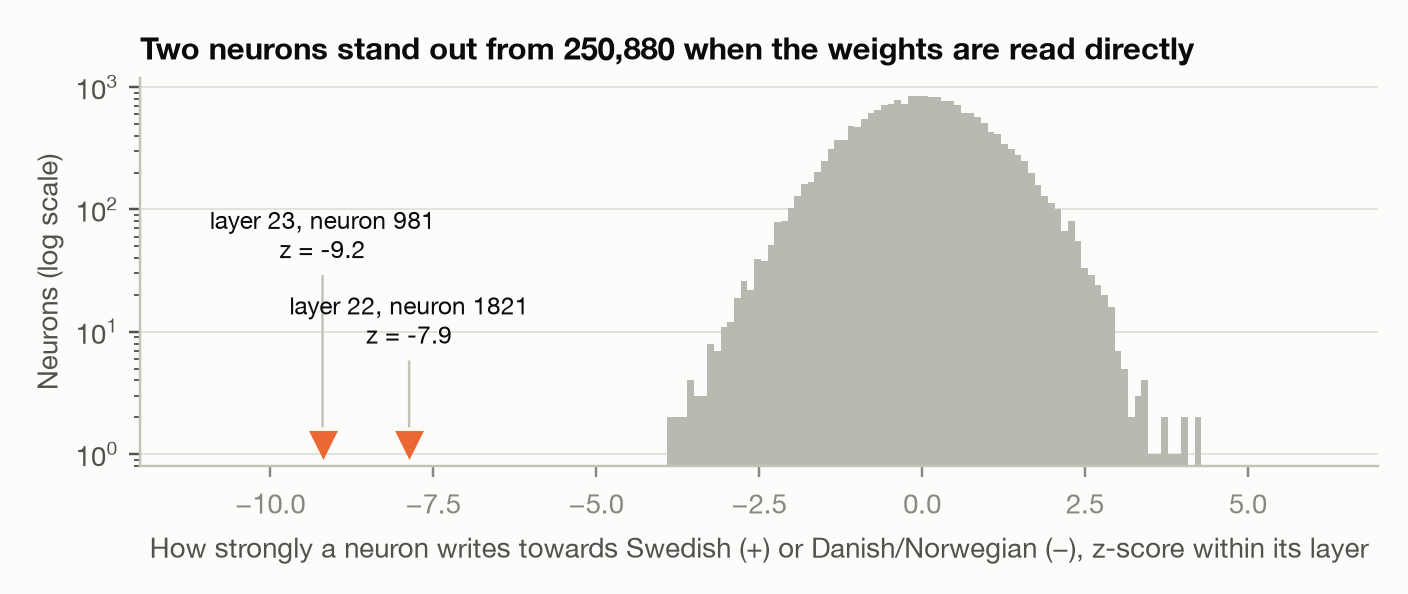
\includegraphics[width=0.74\textwidth]{../figures/fig1_weight_reading.png}
\caption{The screen. Grey: a random sample of 20,000 of the 250,880 neurons.}\label{fig:read}
\end{figure}

\textbf{How surprising is a score of $-9.2$?} Less than the figure suggests. As a calibrated null I built 200 control directions from the same 34 tokens paired at random.
\NullMin\ of them contain a neuron at or beyond $-9.2$, and \NullMinB\ one at or beyond $-7.9$, because a neuron that promotes a single token already produces a large score.
A statistic that rewards consistency across the 17 pairs ranks neuron 981 seventh and neuron 1821 nineteenth of 250,880. With random subsets of 8 of the 17 pairs, the same two neurons are the top two 72\% of the time.
So the screen \emph{nominates candidates}; it does not certify them. The evidence that these two matter is the deletion test, and I did not test the other neurons the consistency statistic would have nominated.

\textbf{Edits and comparisons.} W0, pre-registered: zero the output columns of both neurons (3,072 of 1.54 billion weights). R0: two random neurons in the same layers, 5 seeds.
W1: the same family tuned with feedback on 2,040 dev generations. P1: ``Svara alltid på svenska.'' in the system prompt. S1: activation steering, 9 settings.
F1: LoRA, rank 8, on 80 dev prompts with the model's own Swedish answers as targets.

\textbf{Round-1 data.} Synthetic template--topic prompts with Swedish and English versions; development uses 8 templates and 20 topics; the held-out test uses 20 other topics crossed with the 8 development templates (\code{sv\_A}) and with 8 unseen templates (\code{sv\_B}), 320 prompts.

\textbf{Metrics.} Target: share of answers in Swedish, by the \code{lingua} detector (100\% correct on natural Swedish, English, Danish and Norwegian text). Regression checks: English and Danish prompts,
perplexity on natural text in four languages, degenerate output. Capability check: Swedish grammatical minimal pairs. Intervals: a paired bootstrap that resamples templates and topics separately (Owen's pigeonhole bootstrap),
because prompts are crossed and failures cluster in templates. It measures sensitivity to drawing templates and topics like these, not coverage for Swedish prompts in general.

\section{Round 1}

\begin{table}[H]\footnotesize\centering\setlength{\tabcolsep}{4pt}
\begin{tabular}{@{}lccccccc@{}}
\toprule
 & Swedish & $\Delta$ vs B0 & Fixed / & English & Danish & Swedish & Grammar\\
Condition & answers & [95\% CI], points & broken & \up English & \up Danish & PPL & pairs\\
\midrule
B0 Unedited & 85.0\% & -- & -- & 100\% & 82.5\% & 52.5 & 73.0\%\\
R0 Random 2 neurons (5 seeds) & 85.4\% & $+0.4$ & -- & -- & -- & 52.5 & --\\
\textbf{W0 Both neurons (pre-registered)} & \textbf{91.2\%} & $+6.2$ [$-4.7$, $+18.8$] & 35 / 15 & 100\% & 13.1\% & 56.8 & 72.6\%\\
W0a Only L23/N981 (exploratory) & 96.9\% & $+11.9$ [$+2.8$, $+23.4$] & 38 / 0 & 100\% & 10.0\% & 51.7 & 73.4\%\\
W0b Only L22/N1821 (exploratory) & 20.0\% & $-65.0$ [$-77.8$, $-50.0$] & 3 / 211 & 100\% & 80.0\% & 77.2 & 68.8\%\\
S1 Activation steering (9 settings) & 83.1\% & $-1.9$ [$-7.5$, $+3.8$] & 11 / 17 & 100\% & 77.5\% & 55.4 & 70.0\%\\
F1 LoRA, 80 examples & 99.1\% & $+14.1$ [$+2.8$, $+28.1$] & 47 / 2 & 100\% & 78.8\% & 63.2 & 73.0\%\\
P1 Prompt instruction & 99.4\% & $+14.4$ [$+3.4$, $+28.4$] & 47 / 1 & 74.4\% & 3.8\% & 52.5 & 73.0\%\\
\bottomrule
\end{tabular}
\caption{Round 1, 320 held-out Swedish prompts. Of the 48 unedited failures, 40 are Danish or Norwegian (12.5\%), 5 German, 3 English. ``Fixed / broken'' counts only the Swedish-or-not label.
W1 is absent because feedback tuning selected exactly W0.}\label{tab:main}
\end{table}

\textbf{The pre-registered edit missed.} It cut wrong-language answers from 48 to 28 (41.7\%, where 50\% was required), its interval includes zero, and Swedish perplexity rose 8\% (5\% allowed). H1 and H2 are not met.

\textbf{The pooled number hides a split.} The gain is 81.9\%\up93.8\% on templates seen during development and 88.1\%\up88.8\% on unseen templates. Three templates hold 39 of the 48 unedited failures (Table~\ref{tab:tmpl}).
Feedback tuning on development prompts picked the same edit and scored it 100\% there.

\begin{table}[H]\footnotesize\centering
\begin{tabular}{@{}llccc@{}}
\toprule
Set & Template & Unedited failures (of 20) & W0 fixed / broken & W0a fixed / broken\\
\midrule
seen & Skriv tre meningar om \dots & 13 & 11 / 0 & 12 / 0\\
seen & Kan du berätta lite om \dots? & 11 & 11 / 0 & 11 / 0\\
seen & Ge mig två intressanta fakta om \dots & 5 & 2 / 0 & 4 / 0\\
seen & five other templates & 0 & 0 / 5 & 0 / 0\\
unseen & Skriv en kort dikt om \dots & 15 & 7 / 0 & 7 / 0\\
unseen & Beskriv \dots\ med enkla ord. & 3 & 3 / 5 & 3 / 0\\
unseen & Vilka vanliga missförstånd finns det om \dots? & 1 & 1 / 2 & 1 / 0\\
unseen & five other templates & 0 & 0 / 3 & 0 / 0\\
\bottomrule
\end{tabular}
\caption{Round 1 by template. The poem template fails mostly into German (``Dikt''), which no neuron edit touches.}\label{tab:tmpl}
\end{table}

\textbf{Why deleting both was the wrong edit.} Both neurons' output weights point towards Danish. But on development prompts neuron 981 was active ($+35.5$) only in answers that came out Danish or Norwegian, while neuron 1821 was strongly \emph{negative} ($-19.0$) in answers that came out Swedish.
A negative activation times a Danish-pointing output is a push towards Swedish. In this architecture an activation is a product of two terms and can take either sign, so output weights show what a neuron writes, not when or with which sign it fires.
One batch of 80 forward passes showed this. Section~\ref{sec:prefix} measures it properly.

\textbf{Costs} (Table~\ref{tab:regress}). Under the one-neuron edit, Danish answers to Danish prompts fall from 82.5\% to 10.0\% and Danish perplexity rises 72\%. LoRA removes drift and keeps most Danish answers, but its perplexity rises 20--25\% in Swedish, Danish and Norwegian,
most likely because it was trained on the model's own Swedish. The Swedish prompt instruction over-applies: 26\% of English prompts get Swedish answers.

\begin{table}[H]\footnotesize\centering\setlength{\tabcolsep}{4pt}
\begin{tabular}{@{}lccccccc@{}}
\toprule
 & \multicolumn{4}{c}{Perplexity on natural text} & Danish prompts: & Weights & Model feedback\\
Condition & sv & en & da & no & answers da / sv / no & changed & used to build it\\
\midrule
B0 Unedited & 52.5 & 44.6 & 99.3 & 103.3 & 132 / 4 / 23 & -- & --\\
W0 Both neurons & 56.8 & 44.6 & 173.6 & 119.3 & 21 / 105 / 33 & 3,072 & none\\
W0a Only L23/N981 & 51.7 & 44.6 & 170.6 & 118.6 & 16 / 112 / 31 & 1,536 & 80 dev prompts (sign)\\
W0b Only L22/N1821 & 77.2 & 44.6 & 98.8 & 101.2 & 128 / 2 / 30 & 1,536 & --\\
S1 Steering & 55.4 & 45.4 & 104.1 & 111.4 & 124 / 4 / 24 & none (run-time) & 1,240 dev prompts\\
F1 LoRA & 63.2 & 46.0 & 123.7 & 129.0 & 126 / 18 / 13 & 1.09 million & 80 answers, 60 steps\\
\bottomrule
\end{tabular}
\caption{Round-1 costs. Without three imprecise Danish topic translations (Section~\ref{sec:lang}) the Danish column is 79.4\% unedited and 8.1\% under W0a.}\label{tab:regress}
\end{table}

\textbf{Grammar.} No edit improved grammar-pair accuracy by the pre-registered margin (H3 holds). Accuracy did move down under the harmful edit W0b (73.0\%\up68.8\%). Article gender stays at chance in every condition.
The conclusions are the same on the 195 of 237 pairs whose two sentences have equal token counts, and on a cleaned set without four ambiguous nouns.

\textbf{Notice questions} (added after the pre-registration, on a reviewer's suggestion): 40 questions with a correct code and a distractor. No edit changed factual accuracy on Swedish or English notices (95\% and 100\%).

\section{Round 2: fresh data, more models}\label{sec:r2}

Round 1 left six weaknesses: AI-written prompts, one model and prompt set, a post-hoc headline, a small steering search, a spot-checked reproduction, and an unaudited detector.
Round 2 was pre-registered before any of its test data was run on any model (\code{PREREGISTRATION\_\allowbreak ROUND2.md}). Exploratory additions are in a dated addendum.

\textbf{Fresh data.} \emph{T1}: 320 prompts from 40 new templates $\times$ 8 new topics. \emph{MKQA} (Apple, CC BY-SA 3.0): 300 Natural Questions queries translated by professional translators into Swedish,
the first 150 also in Danish and English; a separate 120-question dev split. \emph{Native grammar pairs}: 200 Talbanken treebank sentences with one indefinite article swapped against the gold gender annotation.

\textbf{A frozen recipe.} (1) Screen the weights as before; candidates are all neurons with $z<-6$, or the two lowest if there are none. (2) Generate 32 tokens for 160 dev prompts and compare each candidate's mean activation
on Danish/Norwegian answers ($a_{da}$) and Swedish answers ($a_{sv}$). Delete a candidate only if $a_{da}>0$ and $a_{sv}>-0.25\,a_{da}$. (3) Zero the output columns of the marked neurons. No per-model choices.

\subsection{Confirmation on the original model}

\begin{table}[H]\footnotesize\centering\setlength{\tabcolsep}{3.5pt}
\resizebox{\textwidth}{!}{%
\begin{tabular}{@{}lcccccccc@{}}
\toprule
 & \multicolumn{2}{c}{T1, new templates} & \multicolumn{3}{c}{MKQA, human-translated} & Danish & English & Grammar\\
Condition & Swedish & da+no & Swedish & $\Delta$ [95\% CI] & da+no / en & \up Danish & \up English & synth.\ / native\\
\midrule
B0 Unedited & 96.6\% & 11 & 50.0\% & -- & 10 / 139 & 47.3\% & 99.3\% & 73.0 / 75.0\\
R Random neuron, 2 seeds & 96.6\% & 11 & 49.7\% & $-0.3$ & 10 / 140 & -- & -- & --\\
\textbf{W0a Only L23/N981 (pre-registered)} & 98.4\% & 5 & 51.0\% & $+1.0$ [$-0.7$, $+2.7$] & 4 / 142 & 16.0\% & 99.3\% & 73.4 / 76.0\\
W0 Both neurons & 93.1\% & 21 & 47.3\% & $-2.7$ [$-5.7$, $+0.3$] & 7 / 150 & 15.3\% & 99.3\% & 72.6 / 75.0\\
P1 ``Svara alltid på svenska.'' & 99.7\% & 1 & 96.3\% & $+46.3$ [$+40.3$, $+52.0$] & 4 / 6 & 13.3\% & 90.7\% & 73.0 / 75.0\\
P2 ``Answer in the user's language'' & 98.4\% & 5 & 78.7\% & $+28.7$ & 9 / 53 & 66.7\% & 99.3\% & --\\
\STwoRow
\bottomrule
\end{tabular}}
\caption{Round 2 on \code{Qwen2.5-1.5B-Instruct}. T1: 320 prompts; MKQA: 300 Swedish questions, 150 Danish, 150 English. P2 is exploratory.}\label{tab:r2}
\end{table}

\begin{itemize}
\item \textbf{C1, repair on new templates: gate not met.} Only 11 of 320 unedited answers (3.4\%) were in the wrong language, below the 5\% gate fixed in advance; they occurred in 6 of the 40 templates, one of which holds 6 of the 11. The edit moved 96.6\%\up98.4\%, $+1.9$ points $[-0.9,+6.6]$.
With at most 3.4 points to gain, this set says how rare the problem is there, and little about repair.
\item \textbf{C2, human-translated questions: held.} The edit changed Swedish answers by $+1.0$ point. The wrong answers there are English (139 of 300), which the edit does not touch.
\item \textbf{C3, Danish regression: held.} Danish answers to Danish questions fell from 47.3\% to 16.0\%.
\item \textbf{C4, no change in grammar: held.} Native pairs 75.0\%\up76.0\%, synthetic 73.0\%\up73.4\%.
\item \textbf{C5, the recipe reproduces the choice: held.} It marks neuron 981 ($a_{da}=+35.8$, $a_{sv}=-0.4$) and keeps neuron 1821 ($+1.0$, $-19.3$). On the discovery model this is a reproducibility check, not a prediction.
\end{itemize}

\textbf{The round-1 edit hurts on fresh prompts.} Deleting both neurons lowers Swedish answers on both new sets (93.1\% and 47.3\%).

\textbf{The failure depends on the prompt set.} The 15\% wrong-language rate of round 1 came from a few templates. On new templates it is 3.4\%; on human-translated questions it is 50\%, and the wrong language is English.
A blinded re-labelling confirmed that the English-labelled answers are English sentences (typically ``I apologize, but I don't have any specific information about \dots'').
Factual accuracy on these questions is too low to analyse jointly (gold answer found in 8.9\% of 202 scorable questions unedited, 9.9\% under P1).

\textbf{Prompting.} The Swedish instruction gives 96.3\% answers in Swedish on MKQA (a measure of answer language, not of correctness: a gold answer appears in about 10\% of answers with or without it) but, as designed, also forces Swedish onto Danish and English users. A request-aware instruction
(``Always answer in the same language as the user's message.'') gives 78.7\% on Swedish questions, raises Danish answers to Danish questions from 47.3\% to 66.7\%, and keeps English at 99.3\%.

\subsection{Is the Danish regression a lost ability or a changed default?}

With the system prompt ``Svar altid på dansk.'' the unedited model answers 83.3\% of Danish questions in Danish. With neuron 981 deleted it manages 28.7\% (and 26.0\% under the request-aware prompt).
So the edit impairs Danish \emph{production} even when Danish is explicitly requested. Danish comprehension was not tested, and the Swedish-or-not score in Table~\ref{tab:main} would not show this cost.

\subsection{Selector or continuation unit? A fixed-prefix test}\label{sec:prefix}

Under greedy decoding, a change in whole-answer language cannot separate ``chooses the language'' from ``keeps Danish going''. Following a reviewer's suggestion I held the text fixed:
14 simple facts, each asked in Swedish and in Danish, each with word-aligned Swedish and Danish answers. The measure is the log-probability margin (Swedish word minus Danish word) for a word outside the 17 screening pairs,
with a neuron zeroed only at the positions that predict that word.

\begin{table}[H]\footnotesize\centering
\resizebox{\textwidth}{!}{%
\begin{tabular}{@{}llccccc@{}}
\toprule
Prompt & Context before the scored word & Margin & Act.\ 981 & $\Delta$ zero N981 [95\% CI] & $\Delta$ zero N1821 [95\% CI] & $\Delta$ control\\
\midrule
Swedish & neutral (shared words only) & $+6.7$ & $-0.3$ & $+0.14$ [$-0.10$, $+0.48$] & $-3.15$ [$-4.91$, $-1.52$] & $-0.09$\\
Swedish & after a Danish prefix & $+5.9$ & $+2.0$ & $+0.07$ [$-0.22$, $+0.44$] & $-3.22$ [$-4.51$, $-1.98$] & $-0.10$\\
Swedish & after a Swedish prefix & $+6.6$ & $-0.8$ & $-0.12$ [$-0.29$, $+0.05$] & $-3.55$ [$-5.06$, $-2.03$] & $+0.04$\\
Danish & neutral (shared words only) & $-7.0$ & $+34.3$ & $+4.54$ [$+2.60$, $+6.52$] & $+0.38$ [$-0.08$, $+0.79$] & $-0.06$\\
Danish & after a Danish prefix & $-5.8$ & $+40.3$ & $+4.74$ [$+3.13$, $+6.45$] & $+0.49$ [$+0.18$, $+0.75$] & $-0.23$\\
\PrefixLastRow
\bottomrule
\end{tabular}}
\caption{Fixed-prefix test, 14 facts per row; margins and changes in nats, positive = towards Swedish. Control: the layer-23 neuron with the closest output-norm $\times$ activation.}\label{tab:prefix}
\end{table}

Neuron 981 is silent on these Swedish prompts and does nothing there, even after a forced Danish prefix. On Danish prompts it is fully active \emph{before the first answer word} and accounts for about 4.5 nats of the preference for Danish.
Neuron 1821 is its mirror image on Swedish prompts. By the rule fixed in the addendum, neuron 981 is not a continuation unit: it acts at the decision point. But it acts on a ``this conversation is Danish'' signal that is already present at that position, computed earlier in the network.
On prompts where the model drifts, that upstream signal is what is wrong. Deleting neuron 981 blocks the expression of the signal, which is why it also blocks Danish when Danish is correct. I had expected a continuation unit (65\%); that expectation was wrong.

\subsection{Survey: the same recipe on three more models}

\begin{table}[H]\footnotesize\centering\setlength{\tabcolsep}{3.5pt}
\resizebox{\textwidth}{!}{%
\begin{tabular}{@{}lcccccccc@{}}
\toprule
 & Screen & Deleted & \multicolumn{2}{c}{T1 Swedish (da+no answers)} & \multicolumn{2}{c}{MKQA Swedish} & \multicolumn{2}{c}{Danish\up Danish}\\
Model & (candidates) & neurons & unedited & recipe edit & unedited & recipe edit & unedited & recipe edit\\
\midrule
Qwen2.5-1.5B & strong (2) & 1 & 96.6\% (11) & 98.4\% (5) & 50.0\% & 51.0\% & 47.3\% & 16.0\%\\
Qwen2.5-0.5B & weak (2) & 1 & 84.1\% (36) & 92.2\% (12) & 69.3\% & 72.7\% & 51.3\% & 40.7\%\\
Qwen3-1.7B & strong (7) & \QwenThreeDel & 96.6\% (9) & 99.4\% (0) & 86.7\% & 88.3\% & 82.0\% & 35.3\%\\
EuroLLM-1.7B & strong (4) & 2 & 99.4\% (2) & 99.7\% (1) & 88.3\% & 88.7\% & 81.3\% & 21.3\%\\
\bottomrule
\end{tabular}}
\caption{The frozen recipe on four models (all Apache-2.0). Random-neuron controls changed T1 by 0.0 points in every model. ``Strong'' = at least one neuron with $z<-6$.}\label{tab:survey}
\end{table}

\begin{figure}[H]\centering
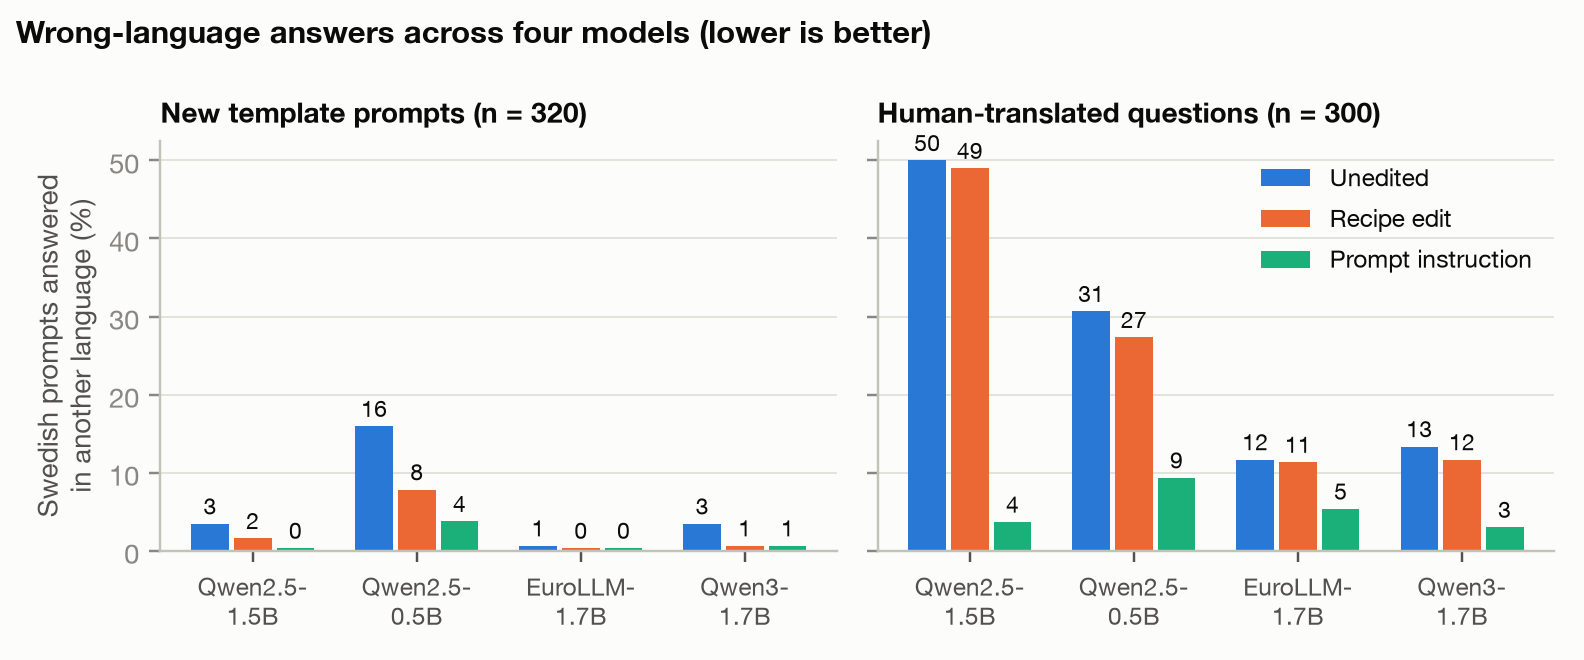
\includegraphics[width=0.86\textwidth]{../figures/fig4_survey.png}
\caption{Wrong-language answers to Swedish prompts in four models.}\label{fig:survey}
\end{figure}

\begin{itemize}
\item \textbf{S-read:} two of the three new models have strong outliers; Qwen2.5-0.5B does not ($z=-5.1$), yet its ``weak'' candidate is the one that works.
\item \textbf{S-drift:} only Qwen2.5-0.5B exceeds 5\% wrong-language answers on new templates (15.9\%). EuroLLM-1.7B, trained on European languages, is at 0.6\% and has far better Swedish (perplexity 23.8, grammar pairs 98\%).
\item \textbf{S-fix:} in the one eligible model, Qwen2.5-0.5B, the recipe cut Danish/Norwegian answers from 36 to 12 and lifted Swedish answers by 8.1 points $[+1.3,+15.9]$, with no change from random neurons. The prediction held in one of one eligible models.
\item \textbf{In every model the edit reduced Danish answers to Danish questions}, by 11 to 60 points. Where a model does not drift, that is the only thing the edit does.
\end{itemize}
The screen-plus-sign recipe therefore generalises as a way to find neurons that carry Danish output in small models. It does not generalise as a way to make a model answer in Swedish, because drift into Danish is not the main failure outside my first prompt set.

\subsection{A larger steering search}
\STwoText

\subsection{Checks of the language material and the detector}\label{sec:lang}

\textbf{Native sources.} All 43 noun genders, 22 definite forms and 10 adjective paradigms agree with Swedish Wiktionary. In Språkbanken's Swedish Wikipedia corpus the grammatical variant outnumbers the ungrammatical one in
30 of 31 article patterns, 20 of 20 adjective patterns (112,367 against 28 hits), 21 of 21 definiteness patterns, 7 of 8 verb-second patterns and both negation patterns.
The exception, \emph{kort}, is also an adjective; with three nouns that Wiktionary lists under both genders (\emph{hus}, \emph{tåg}, \emph{fotografi}) it is dropped in a cleaned set of 223 pairs, which gives the same results.
A spell-checker (LanguageTool) flags nothing in 960 Swedish prompts and two rare but attested compounds in the Danish ones.
The ``ungrammatical'' variants are judged against contemporary standard written Swedish; verb-third order of the kind ``Igår hon köpte \dots'' is attested in urban vernacular Swedish.

\textbf{Danish translations.} A reviewer found three imprecise topic words (\emph{hjemmearbejde}, \emph{genbrug}, \emph{ligestilling}). Dropping those 24 prompts changes the round-1 Danish result from 82.5\%\up10.0\% to 79.4\%\up8.1\%.
Round 2 uses professionally translated Danish and shows the same regression.

\textbf{Detector audit.} I re-labelled 48 shuffled answers with condition and detector label hidden (an AI agent's reading, not a human's). Agreement on Swedish-or-not was 90\%.
The disagreements are one-sided: of 8 round-1 answers the detector called ``broken'' under the two-neuron edit, I read 4 as Swedish and 2 as Swedish mixed with Norwegian. So the detector overstates how much that edit breaks, and understates mixing.
A detector-free count of function words gives the same ranking of conditions, but it reuses the screening vocabulary and is not independent evidence.

\subsection{Reproduction}
\ReproText

\section{Scorecard}

\begin{table}[H]\footnotesize\centering
\begin{tabularx}{\textwidth}{@{}l>{\raggedright\arraybackslash}X l@{}}
\toprule
 & Prediction & Outcome\\
\midrule
H1 & Some pre-registered edit halves drift within the regression limits & Not met (41.7\% cut, perplexity $+8\%$)\\
H2 & The zero-forward-pass edit does so & Not met\\
H3 & No edit improves Swedish grammar or perplexity & Held\\
H4 & Diagnostic: does the edit suppress Danish? & Yes, in every model\\
C1 & One-neuron edit halves wrong-language answers on new templates & Gate not met (3.4\% baseline)\\
C2 & It changes Swedish answers on human-translated questions by under 5 points & Held ($+1.0$)\\
C3 & Danish answers to Danish questions fall by more than half & Held (47.3\%\up16.0\%)\\
C4 & Grammar pairs move by under 3 points & Held\\
C5 & The recipe reproduces the choice of neuron & Held\\
S-read & Strong outlier in each new model & 2 of 3\\
S-drift & New models drift at least 5\% on new templates & 1 of 3\\
S-fix & Recipe halves Danish/Norwegian answers where they occur & 1 of 1 eligible\\
C6 & A larger steering search halves wrong-language answers on new templates & \CSixOutcome\\
\bottomrule
\end{tabularx}
\end{table}

\section{Related work and ways forward}

A short survey (papers opened and checked; the fuller survey was cut short) places these results:
\begin{itemize}
\item \textbf{Wrong-language answers are common and prompt-dependent.} Marchisio et al.\ (arXiv 2406.20052) benchmark this ``language confusion'' and report that it is ``partially mitigated via few-shot prompting, multilingual SFT and preference tuning''.
Their benchmark has no Scandinavian language and measures drift to English. NorEval (arXiv 2504.07749) reports language switching in 23 of 100 hand-checked Norwegian outputs.
\item \textbf{A few neurons can steer output language, at a cost to that language.} Tang et al.\ (arXiv 2402.16438), Kojima et al.\ (2404.02431) and Gurgurov et al.\ (2507.22608) find language-selective neurons from activations; the last reports that Swedish and Danish share about three quarters of theirs in an 8-billion-weight model.
Published sets number hundreds to thousands of neurons, and single-neuron effects shrink with model size (Gurnee et al., 2305.01610). I found no prior work that identifies language neurons from weights alone.
\item \textbf{Fixes that avoid removing a language.} Nie et al.\ (2505.16538) locate ``confusion points'' in the final layers and edit neurons chosen by comparison with a multilingually tuned counterpart. Sterz et al.\ (ReCoVeR, 2509.14814) build steering vectors from a multi-parallel corpus and report retained task performance.
Ji et al.\ (Smoothie-Qwen, 2507.05686) adjust token-level output probabilities without retraining.
\item \textbf{Measurement.} Fedorova et al.\ (SLIDE, 2502.06692) show that Scandinavian sentences often cannot be assigned to a single language and provide multi-label identification, which would replace the detector used here.
\end{itemize}

\section{Recommendation}

\textbf{On the available evidence, SE.LLMA should not deploy this neuron ablation.} Where it changed behaviour it did so by suppressing Danish output, it added no Swedish competence, and on human-translated questions it did not change how often the model answers in Swedish. This is evidence about one edit family on four small models, not about weight editing in general.

\textbf{Measure first.} Add \emph{correct answer in the requested language} to SE.LLMA's evaluation, with human-written prompts and a multi-label Scandinavian language identifier. Wrong-language rates here ranged from 0.6\% to 50\% depending on the model and the prompt set, so a single synthetic set would have misled, and did mislead me in round 1.

\textbf{Then the cheap and the standard fixes.} Request-aware prompting recovered most Swedish answers without harming Danish or English. Fine-tuning on real Swedish text is what SE.LLMA already plans; the 80-example LoRA here suggests that little data is needed for answer language, and its perplexity cost shows why the data should be real Swedish.

\textbf{Most informative next experiment.} A prospective test of weight screening as a diagnostic. Screen base models and their Swedish fine-tunes \emph{before} measuring them, and check (1) whether the screen predicts which checkpoints drift into a sibling language, and (2) whether fine-tuning changes the neurons it flags.
This would test ``auditing without evaluation'', the article's most valuable claim, on checkpoints where the answer is not yet known. A second, mechanistic step is to find where the wrong ``this is Danish'' signal is computed, upstream of layer 22.

\section{Limitations}
\begin{itemize}
\item \textbf{Four small models}, greedy decoding, 48-token answers, one seed. Neuron indices are specific to each checkpoint. Larger models were not tested, and the literature suggests single-neuron effects weaken with size.
\item \textbf{The discovery estimate is inflated by selection.} The 96.9\% of round 1 was found after looking at the data. Its confirmation set had too little baseline failure to settle efficacy on the original model; the only confirmatory evidence of efficacy is from Qwen2.5-0.5B.
\item \textbf{The screen is not statistically specific} (11\% of control directions match its strongest score), and its other candidates were not tested.
\item \textbf{No native speaker has reviewed the synthetic material.} Checks against Wiktionary, corpus counts and a spell-checker, and the use of human-translated and native text in round 2, reduce but do not remove this.
\item \textbf{Language labels are automatic}, audited only by an AI agent on 48 answers. Mixed answers are not scored as such.
\item \textbf{MKQA is translated open-domain QA}; its 46\% English rate belongs to this checkpoint and prompt format. Short factual answers were rare (median answer length about 30 words), so labels are not driven by names and dates, but the estimate should not be read as a general rate.
\item \textbf{LoRA was not rerun in round 2}, and it was trained on the model's own Swedish.
\end{itemize}

\section{Reproducibility and AI use}
Code, both pre-registrations with their commit history, every raw model output and per-item score are in the repository. \code{./run\_all.sh} reproduces round 1 and \code{./run\_round2.sh} round 2; the analysis scripts rebuild all tables and figures from the committed results in seconds.
Model revisions, library versions and seeds are pinned.

An AI coding agent (Claude Code) did the weight screening, wrote the code, ran the experiments and drafted this report. A second AI assistant reviewed the plan and the round-1 results;
its review led to the fixed-prefix test, the calibrated null, the per-template table, the request-aware prompt and several corrections of wording. Details are in \code{AI\_USAGE.md}.

\end{document}
